%-----------------------------------------------------------------------
%
%   UFRJ  - Universidade Federal do Rio de Janeiro
%   COPPE - Coordena��o dos Programas de P�s-gradua��o em Engenharia
%   PEE   - Programa de Engenharia El�trica
%
%   COE-835  Controle adaptativo
%
%   Relat�rio da simula��o
%                                                         Ramon R. Costa
%                                                         05/out/09, Rio
%-----------------------------------------------------------------------
\documentclass[11pt,a4paper]{article}
\usepackage[latin1]{inputenc} %pacote para utilizar palavras acentuadas
\usepackage{amsmath,amssymb}  %pacotes do AMS
\usepackage{latexsym}         %pacote para incluir s�mbolos (ex.\Box)
\usepackage{fancybox,fancyhdr}%pacote com frescuras
\usepackage{graphicx}         %pacote para incluir figuras tipo eps
\usepackage[portuguese]{babel}
\usepackage{xcolor}
\usepackage{float} 
\usepackage{epstopdf}
\usepackage[inline]{enumitem}
\usepackage[a4paper]{hyperref}% Make sure it comes last of your loaded packages
\hypersetup{
  verbose,
  plainpages=false,
  bookmarks=true,
  colorlinks=true,
  linkcolor=blue
}
     
%----------------------------------------------------------------------
%
%   Macros utilizados no LATEX
%                                                       Ramon R. Costa
%                                                       13/out/17, Rio
%----------------------------------------------------------------------
\newcount\m
\newcount\n

\def\twodigits#1{\ifnum #1<10 0\fi \number#1}

\def\hours{\n=\time \divide\n 60
    \m=-\n \multiply\m 60 \advance\m \time
    \twodigits\n:\twodigits\m}

\def\hora{\hours}

\def\fim{
  \medskip
  \begin{center}
    \rule[1mm]{30mm}{0.14mm}$\diamond$\rule[1mm]{30mm}{0.14mm}
  \end{center}
}

%----------------------------------------------------------------------
% A4 paper size & margins
\setlength {\textheight}    {25cm}%
\setlength {\textwidth}     {17.5cm}%
\setlength {\parindent}     {0mm}%
\setlength {\parskip}       {1mm}%
\setlength {\topmargin}     {-14mm}%
\setlength {\oddsidemargin} {-6mm}%
\setlength {\evensidemargin}{-6mm}%
\setlength {\columnsep}     {6mm}%

%----------------------------------------------------------------------
\def\codigo{COE-835}
\def\disciplina{Controle adaptativo}
\def\periodo{3o. período/2017}
\def\professor{Ramon}

\newcommand{\BOX}[1]{
  \framebox{{\color{magenta}\rule[-3mm]{1mm}{9mm}} ~~$\displaystyle
  \begin{aligned} #1 \end{aligned}$~~}\pagestyle{plain}
}

\newcommand{\RED}[1]{\colorbox{white}{\textcolor{red}{#1}}}
%\newcommand{\WoR}[1]{\colorbox{red}{\textcolor{white}{#1}}}
\newcommand{\BLU}[1]{\colorbox{white}{\textcolor{blue}{#1}}}
\newcommand{\GRE}[1]{\colorbox{green}{\textcolor{black}{#1}}}
\newcommand{\HI}[1]{\colorbox{yellow}{\textcolor{black}{#1}}}  %% Highlithed text

\newcommand{\estrela}[1]{
  \def\TXT{\RED{$\bigstar$ }}
  \hspace*{5mm}\TXT \hfill
  \parbox[t]{ \textwidth - \widthof{\TXT} - 5mm}{#1}
  \par
}

\def\Ltwo{\mbox{${\mathcal L}_2$}}
\def\Linf{\mbox{${\mathcal L}_\infty$}}

\newcommand{\sign}{\mbox{sign}}

\newcommand{\equacao}[2]{
  \makebox[40mm][l]{#1 \dotfill}: \quad \parbox[t]{8cm}
	{\begin{equation} \displaystyle
  \begin{aligned}
    #2
  \end{aligned} \end{equation}} \\
}

\newcommand{\sref}[1]{Section~\ref{#1}}
\newcommand{\fref}[1]{Fig.~\ref{#1}}
\newcommand{\tref}[1]{Table~\ref{#1}}
\newcommand{\thref}[1]{Theorem~\ref{#1}}
\newcommand{\aref}[1]{Assumption~\ref{#1}}
\newcommand{\norm}[1]{\left\lVert#1\right\rVert}
%\renewcommand{\qedsymbol}{}
\newcommand{\rev}[1]{{\color{red}#1}}
%\newcommand{\mat}[1]{\begin{bmatrix}#1\end{bmatrix}}

\newtheorem{remark}{Remark}
\newtheorem{lemma}{Lema}

%----------------------------------------------------------------------


%Set normal paragraph spacing
\setlength\parindent{24pt}

\begin{document}
%---------------------------------------------------------------------
\pagestyle{fancy}%
\renewcommand{\headrulewidth}  {0.4pt}%
\renewcommand{\footrulewidth}  {0.4pt}%
\lhead{\bfseries{Relat�rio do Trabalho 5}}%
\chead{}%
\rhead{\bfseries\thepage}%
\lfoot{}%
\cfoot{}%
\rfoot{[\hours] \quad \today}%
%---------------------------------------------------------------------
\begin{center}
  \huge{COE-835  Controle  adaptativo}  \\[20mm]

  \Large{Trabalho 5} \\[20mm]
\end{center}

\textbf{Grupo:} \quad \parbox[t]{10cm}{
Guilherme Pires Sales de Carvalho \\[2mm]
Matheus Ferreira dos Reis \\[2mm]
Renan Salles de Freitas \\[10mm]
}

\textbf{Algoritmo:} \quad \HI{MRAC Direto} ($n^* = 1$) \\[2mm]

\bigskip%
\textbf{Caso}: \quad \parbox[t]{10cm}{
  $n = 2, 3$ \quad (ordem da planta) \\[2mm]
  $n^* = 1$ \quad (grau relativo) \\[2mm]
  $n_p = 4, 6$ \quad (\# de par�metros) \\[15mm]
}

%---------------------------------------------------------------------
\tableofcontents
\newpage
%---------------------------------------------------------------------
%---------------------------------------------------------------------
\section{MRAC direto}

O controle adaptativo de modelo de refer�ncia (MRAC) � um m�todo de controle
adaptativo com uma funda��o teoria rigorosa e sistem�tica, possui promissora e
atraente perspectiva de aplica��o, e seu projeto � simples e conciso. O objetivo
do MRAC � garantir que a sa�da de um sistema controlado (planta)) seja igual a
sa�da de um dado modelo de refer�ncia, e a estabilidade do ssitema em malha
fechada.Quando os par�metros da planta s�o desconhecidos, leis adaptativas s�o
necess�rias para a atualiza��o dos par�metros.

Considere um sistema linear invariante no tempo descrito pela equa��o
diferencial (Eq. \ref{eq:planta}):
%
\begin{equation}
P(s) \, [y](t) = Z(s) \, [u](t),
\label{eq:planta}
\end{equation}

onde $y(t) \in \mathbb{R}$ e $u(t) \in \mathbb{R}$ s�o os sinais medidos de
sa�da e entrada do sistema, sendo:
%
\begin{gather}
P(s) = s^n + p_{n-1}s^{n-1}+\ldots + p_1s+p_0\,\\
Z(s) = z_ms^m + z_{m-1}s^{m-1}+\ldots + z_1s+z_0 \,,
\label{eq:poly}
\end{gather}
%
os polin�mios em $s$, com $s$ sendo o operador de diferencial
$s[x](t)=\dot{x}(t)$. $p_i$, $i = 0,1,\ldots,n-1$ e $z_i$, $i=0,1,\ldots,m$ ($n>m$) s�o os par�metros desconhecidos da planta.


O objetivo do controle �: dado um modelo de refer�ncia, descrito como

\begin{equation}
P_m(s)[y_m](t) = r(t),
\end{equation}

onde $P_m(s)$ � um polin�mio est�vel m�nico e $r(t)$ � a entrada de refer�ncia
limitada, encontrar uma lei de controle $u(t)$ tal que todo o sistema de malha
fechada produza sinais limitados e a sa�da da planta $y(t)$ rastreie o modelo
de refer�ncia $y_m(t)$ assintoticamente. A estrutura exige algumas premissas:
\begin{enumerate}
  \item $Z(s)$ � um polin�mio est�vel;
  \item O sinal de $k_p$ � conhecido;
  \item O grau relativo da planta � conhecido;
  \item A ordem da planta � conhecida.
\end{enumerate}

A estrutura do controlador � 2DOF, como pode ser visto na figura
\ref{mrac}. Escolhe-se ent�o um polin�mio est�vel $\Lambda(s) =
s^n+\lambda_{n-1}s^{n-1}+\ldots+\lambda_1s+\lambda_0$ para filtrar a entrada e a
sa�da da planta com o filtro $\frac{1}{\Lambda(s)}$. A equa;�o do controlador
]e descrita como:
\begin{equation}
u(t) = \theta_1^\intercal\omega_1(t)+\theta_2^\intercal\omega_2(t)+\theta_n
y(t)+ \theta_{2n} r(t),
\end{equation}

onde o filtro � descrito pela realiza��o de estados:

\begin{gather}
\dot{\omega}_1(t) = A_\lambda \, \omega_1(t) + bu(t)\,,\\
\dot{\omega}_2(t) = A_\lambda \, \omega_2(t) + by(t)\,,
\label{eq:statespace}
\end{gather}
%
onde $\omega_1(t) \in \mathbb{R}^n$, $\omega_2(t) \in \mathbb{R}^n$ e:
%
\begin{equation}
A_\lambda = 
\begin{bmatrix}
    0      & 1      & 0      & \dots  & 0      & 0      \\
    0      & 0      & 1      & 0      & \dots  & 0      \\
    \vdots & \vdots & \vdots & \vdots & \vdots & \vdots \\
    0      & 0      & \dots  & \dots  & 0      & 1      \\
    -\lambda_0 & -\lambda_1 & \dots & \dots & -\lambda_{n-2} & -\lambda_{n-1} 
\end{bmatrix}
\in \mathbb{R}^{n \times n} \,, \quad b =
\begin{bmatrix}
    0  \\
    \vdots  \\
    0 \\
    1 \\ 
\end{bmatrix}
\in \mathbb{R}^n \,.
\label{eq:statespace}
\end{equation}

\begin{figure}[H]
  \centering
  
\includegraphics[width=12cm]{figs/mrac.png}
  \caption{Estrutura MRAC.}
  \label{mrac} 
\end{figure}

Os valores ideais para o controle $\theta^*$ podem ser obtidos como j�
descrito no trabalho 4, se os par�metros da planta fossem conhecidos. Como n�o �
o caso, consideramos $\theta$ como uma estimativa dos par�metros ideais e
formulamos a lei de controle:

\begin{gather}
u(t) = \theta^\intercal\omega, \\
\omega(t) = \left[\omega_1(t)^\intercal \quad y(t) \quad \omega_2(t)^\intercal
\quad r(t)\right]^\intercal, \\
\theta = \left[\theta_1 \quad \theta_n \quad \theta_2 \quad \theta_{2n}\right]
\end{gather}

Definimos o erro como $e(t) = y(t) - y_m(t)$, e � poss�vel demonstrar por
Lyapunov que, variando $\theta$ pela lei

\begin{equation}
\dot{\theta}(t) = -\textrm{sign}[k_p]\Gamma\omega(t)e(t),
\end{equation}

o erro converge assintoticamente para zero, quando $\Gamma =
\Gamma^\intercal > 0$ � uma matrix de ganhos positiva definida.

Neste trabalho, ser�o consideradas plantas de segunda e terceira ordens com grau
relativo 1 ($n^*=1$). Iremos simular e discutir o comportamento do erro e das
sa�das para varia��es das condi��es iniciais dos par�metros estimados
($\theta(0)$) e da planta ($y(0)$), do ganho de adapta��o $\Gamma$ e para
diferentes par�metros da planta e modelo.

\section{Implementa��o}


%---------------------------------------------------------------------
\section{Resultados das simula��es}

%Simula��o utilizando \HI{\texttt{Matlab/Simulink}}.

%\subsection{Gradiente Normalizado}

Nas simula��es, procuramos avaliar o comportamento do sistema para as seguintes condi��es:
%
\begin{enumerate*}[label=(\roman*)]
\item condi��es iniciais $\theta(0)$ e $y(0)$;
\item Par�metros da planta e do modelo;
\item ganho de adapta��o $\Gamma$.
\end{enumerate*}

Apresentaremos os resultados obtidos atrav�s de simula��es no ambiente \HI{\texttt{Matlab/Simulink}} e os discutiremos na pr�xima se��o.

\subsection{Simula��o \#1}

Inicialmente, desejamos verificar o comportamento do sistema para varia��es nas
condi��es iniciais.

\bigskip

\textbf{\underline{Simula��o 1.1}: sistema de 2$^\text{a}$ ordem, $\theta(0)$}
%
\begin{align*}
  y &= \frac{s+1}{s^2+4s+4}u\,,  &  y_m &= \frac{1}{s+1}r\,, & \Lambda &=
  s+1,\\ \theta(0) &= \HI{0} \, \textrm{e} \, \HI{1}\,, & y(0) &= 5 \,, &
  \gamma &= 10 \, \textbf{I}_4\,, \\ r &= 10\textrm{sin}(0.63t) +
  25\textrm{sin}(4.5t) \, .
\end{align*}

\begin{figure}[H]
  \centering
  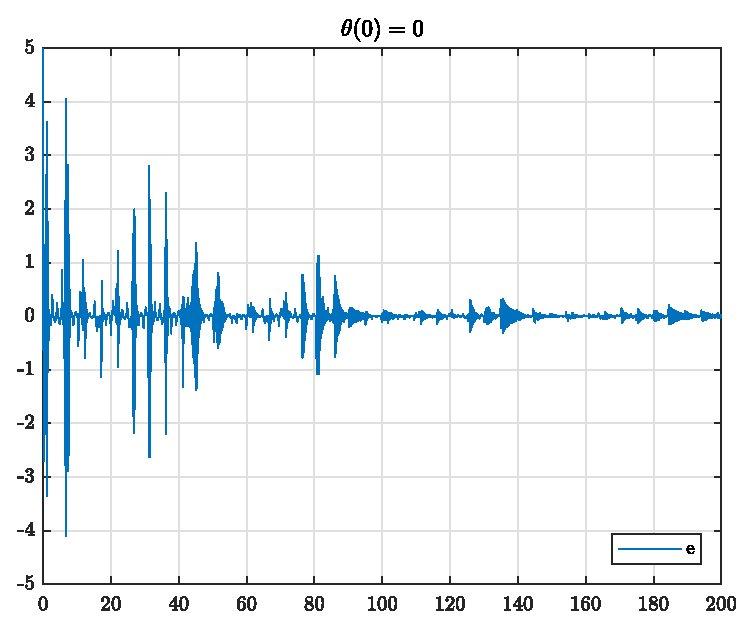
\includegraphics[width=12cm]{figs/en2t0.eps} 
\end{figure}

\begin{figure}[H]
  \centering
  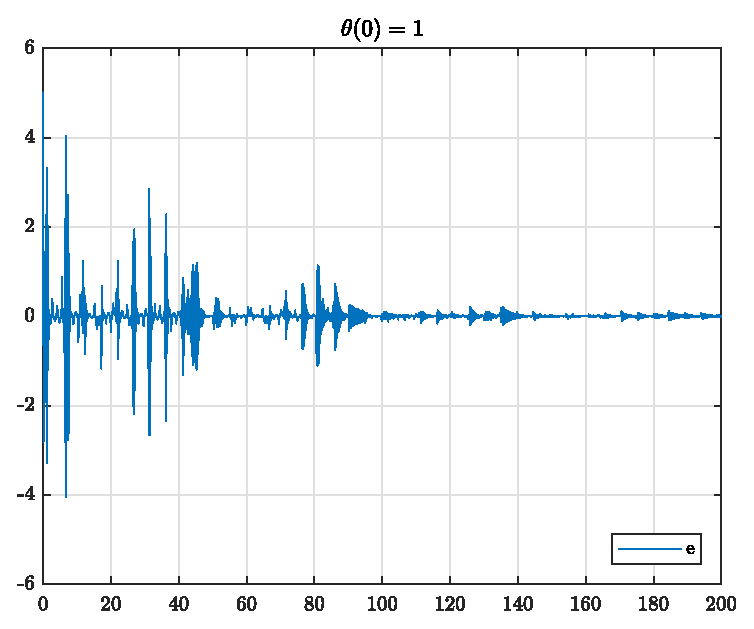
\includegraphics[width=12cm]{figs/en2t1.eps} 
\end{figure}

\begin{figure}[H]
  \centering
  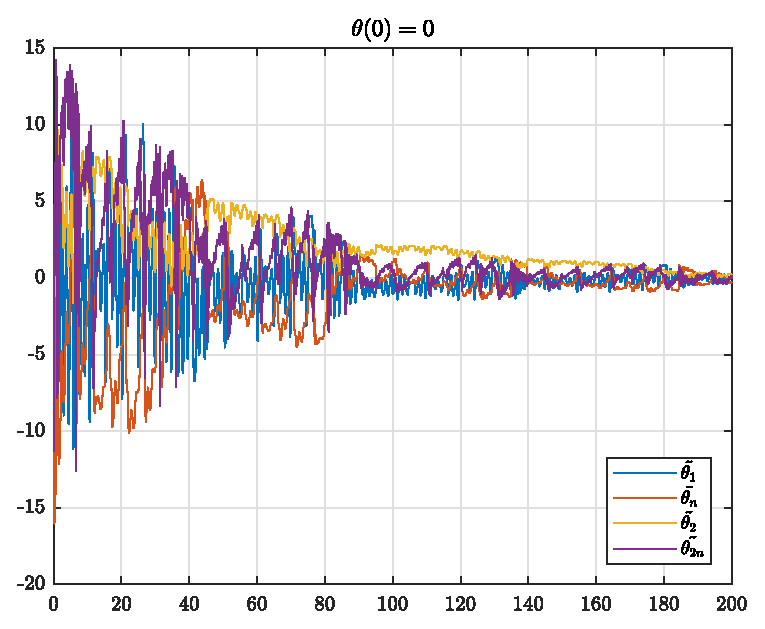
\includegraphics[width=12cm]{figs/tiln2t0.eps} 
\end{figure}

\begin{figure}[H]
  \centering
  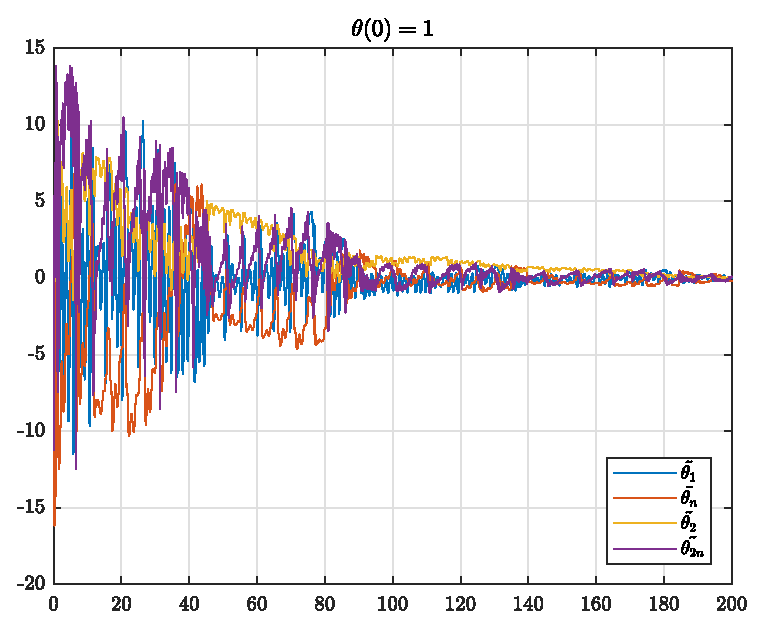
\includegraphics[width=12cm]{figs/tiln2t1.eps} 
\end{figure}

\textbf{\underline{Simula��o 1.2}: sistema de 3$^\text{a}$ ordem, $\theta(0)$}
%

\textbf{\underline{Simula��o 1.3}: sistema de 2$^\text{a}$ ordem, $y(0)$}
%
\begin{align*}
  y &= \frac{s+1}{s^2+4s+4}u\,,  &  y_m &= \frac{1}{s+1}r\,, & \Lambda &=
  s+1,\\ \theta(0) &= 0 \,, & y(0) &= \HI{0} \text{e} \HI{5} \,, &
  \gamma &= 20 \, \textbf{I}_4\,, \\ r &= 10\textrm{sin}(0.63t) +
  25\textrm{sin}(4.5t) \, .
\end{align*}

\begin{figure}[H]
  \centering
  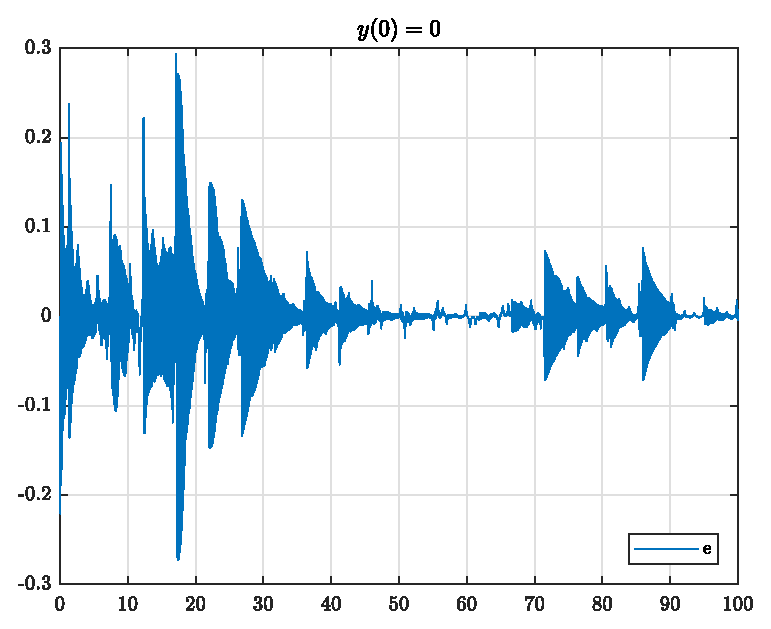
\includegraphics[width=12cm]{figs/en2y0.eps} 
\end{figure}

\begin{figure}[H]
  \centering
  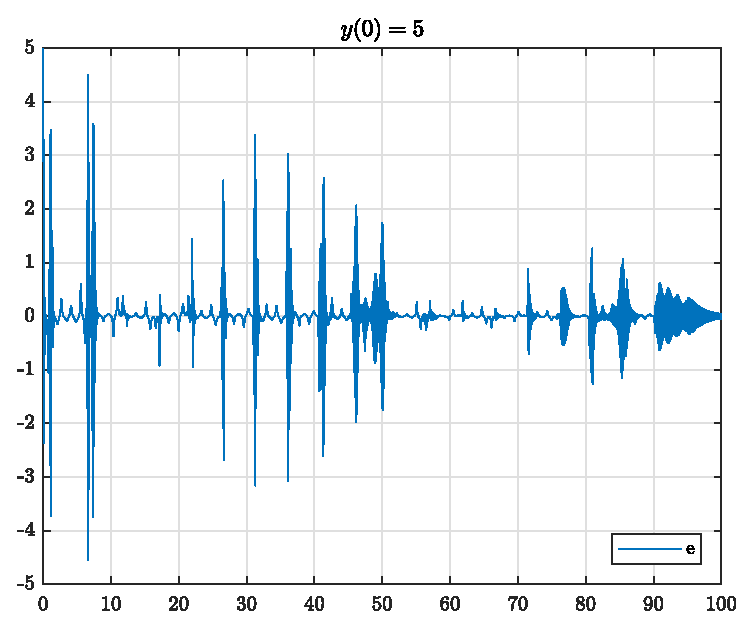
\includegraphics[width=12cm]{figs/en2y5.eps} 
\end{figure}

\begin{figure}[H]
  \centering
  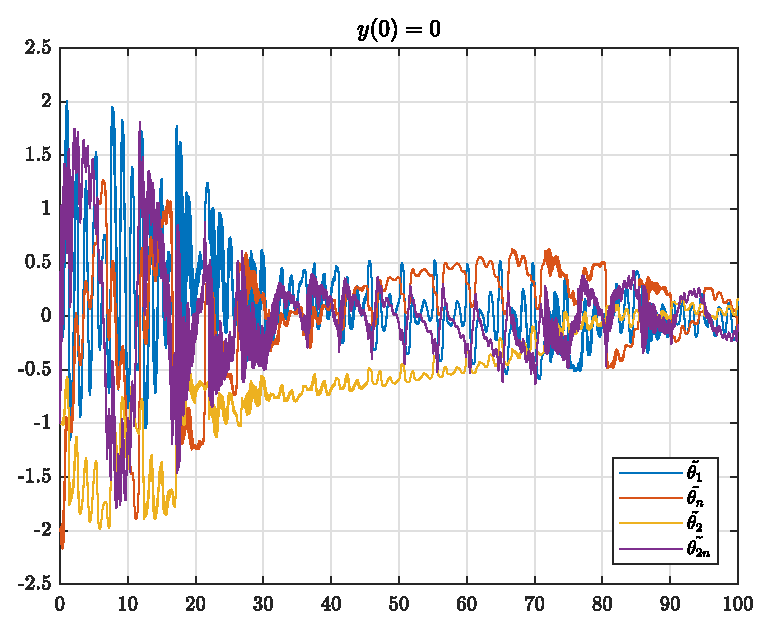
\includegraphics[width=12cm]{figs/tiln2y0.eps} 
\end{figure}

\begin{figure}[H]
  \centering
  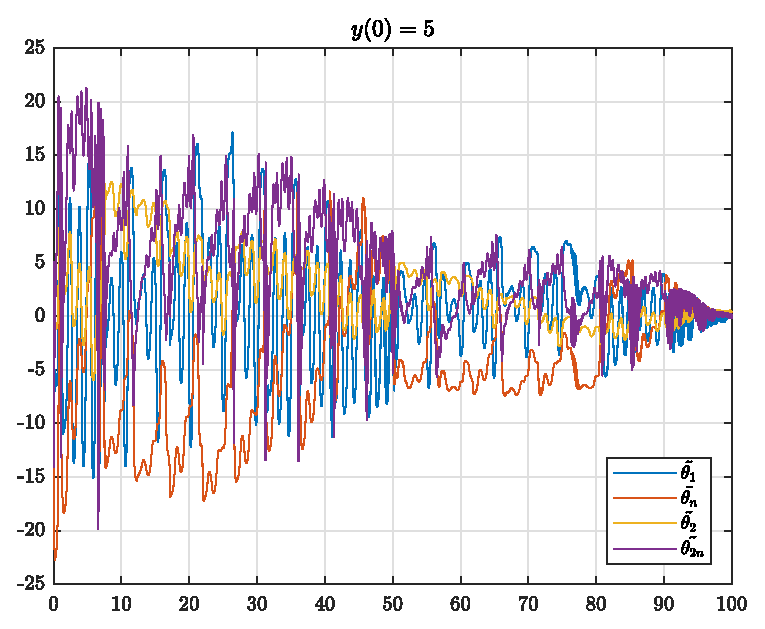
\includegraphics[width=12cm]{figs/tiln2y5.eps} 
\end{figure}

\textbf{\underline{Simula��o 1.4}: sistema de 3$^\text{a}$ ordem, $y(0)$}

% -----------------------------------------------------------------------------

\subsection{Simula��o \#2}

Verificamos o comportamento do sistema para varia��es no par�metro de adapta��o
$\Gamma$.

\bigskip

\textbf{\underline{Simula��o 2.1}: sistema de 2$^\text{a}$ ordem}
%
\begin{align*}
  y &= \frac{s+1}{s^2+4s+4}u\,,  &  y_m &= \frac{1}{s+1}r\,, & \Lambda &=
  s+1,\\ \theta(0) &= 0 \,, & y(0) &= 0 \,, &
  \gamma &= \HI{1} \, \textbf{I}_4 \text{e} \HI{20} \, \textbf{I}_4\,, \\ r &=
  10\textrm{sin}(0.63t) + 25\textrm{sin}(4.5t) \, .
\end{align*}

\begin{figure}[H]
  \centering
  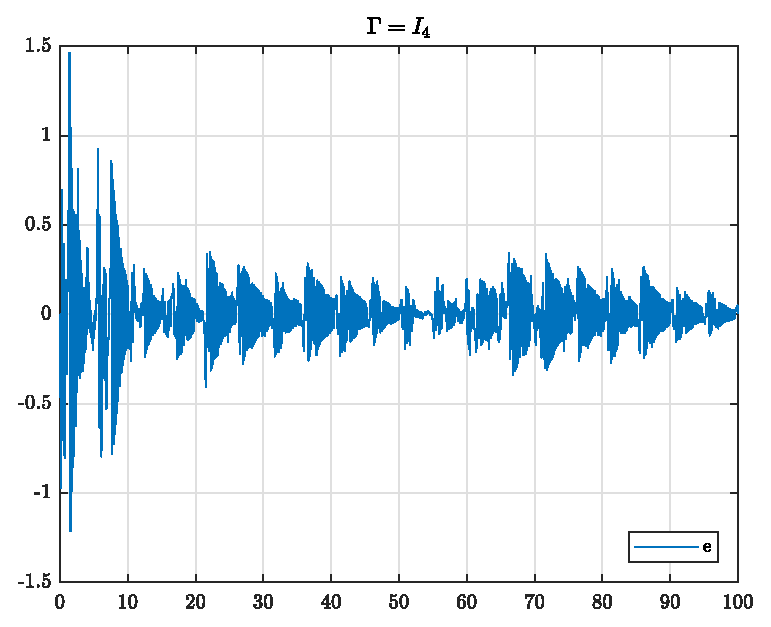
\includegraphics[width=12cm]{figs/en2gamma1.eps} 
\end{figure}

\begin{figure}[H]
  \centering
  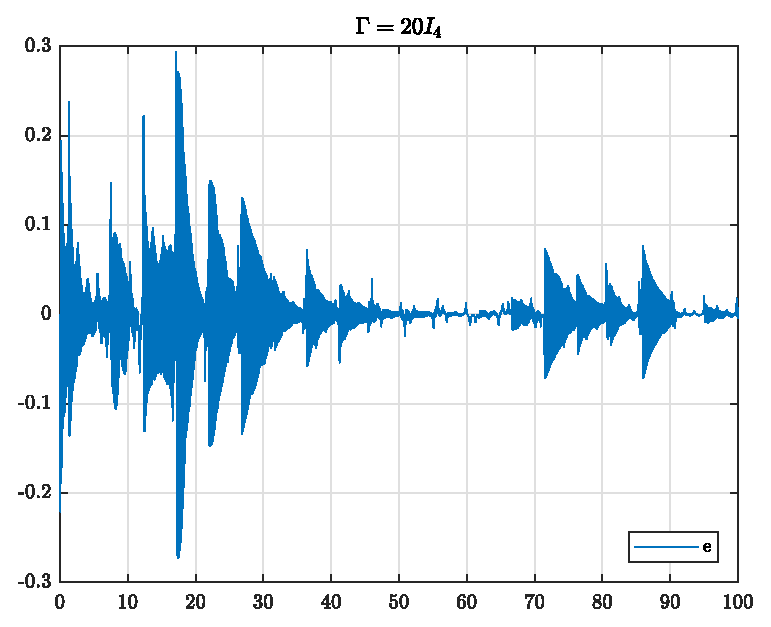
\includegraphics[width=12cm]{figs/en2gamma20.eps} 
\end{figure}

\begin{figure}[H]
  \centering
  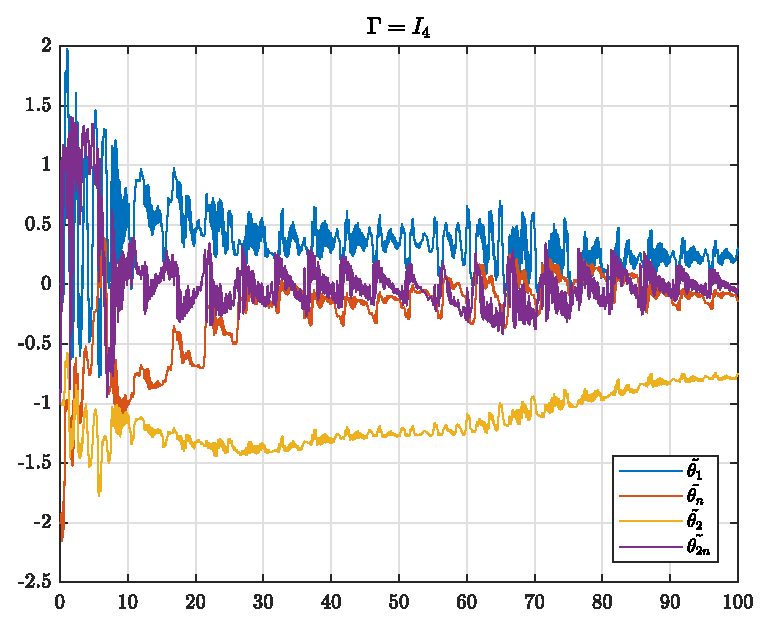
\includegraphics[width=12cm]{figs/tiln2gamma1.eps} 
\end{figure}

\begin{figure}[H]
  \centering
  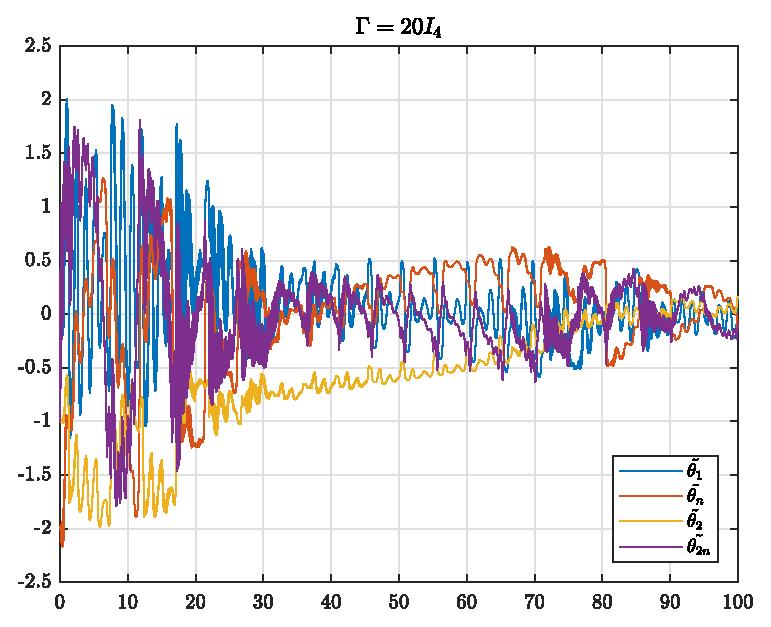
\includegraphics[width=12cm]{figs/tiln2gamma20.eps} 
\end{figure}

\textbf{\underline{Simula��o 2.2}: sistema de 3$^\text{a}$ ordem}
%
% -----------------------------------------------------------------------------

\subsection{Simula��o \#3}

Verificamos o comportamento do sistema para varia��es na planta e modelo.

\bigskip

\textbf{\underline{Simula��o 3.1}: sistema de 2$^\text{a}$ ordem, planta}
%
\begin{align*}
  y &= \frac{s+1}{s^2+4s+4}u\, \text{e} \frac{s+1}{s^2-4s+4}u\,,  &  y_m &=
  \frac{1}{s+1}r\,, & \Lambda &= s+1,\\ \theta(0) &= 0 \,, & y(0) &= 0 \,, &
  \gamma &= 20 \, \textbf{I}_4\,, \\ r &=
  10\textrm{sin}(0.63t) + 25\textrm{sin}(4.5t) \, .
\end{align*}

\begin{figure}[H]
  \centering
  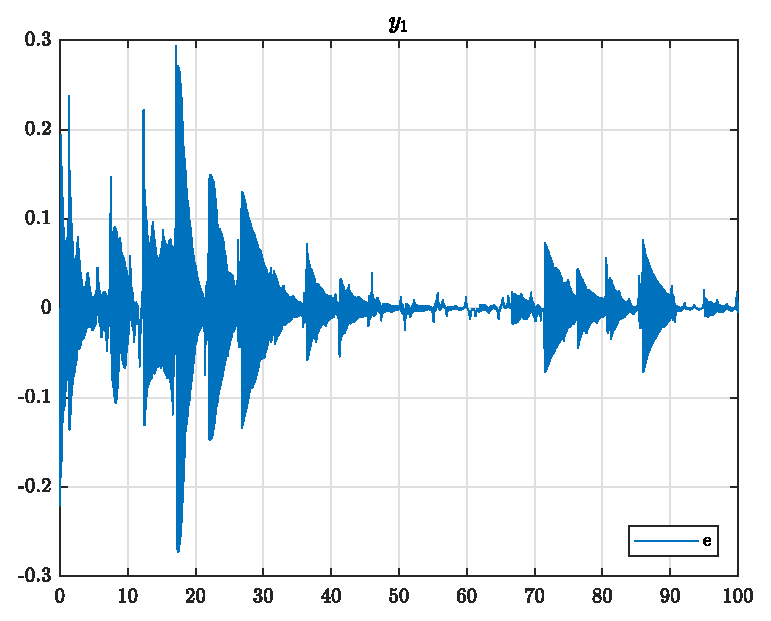
\includegraphics[width=12cm]{figs/en2yp1.eps} 
\end{figure}

\begin{figure}[H]
  \centering
  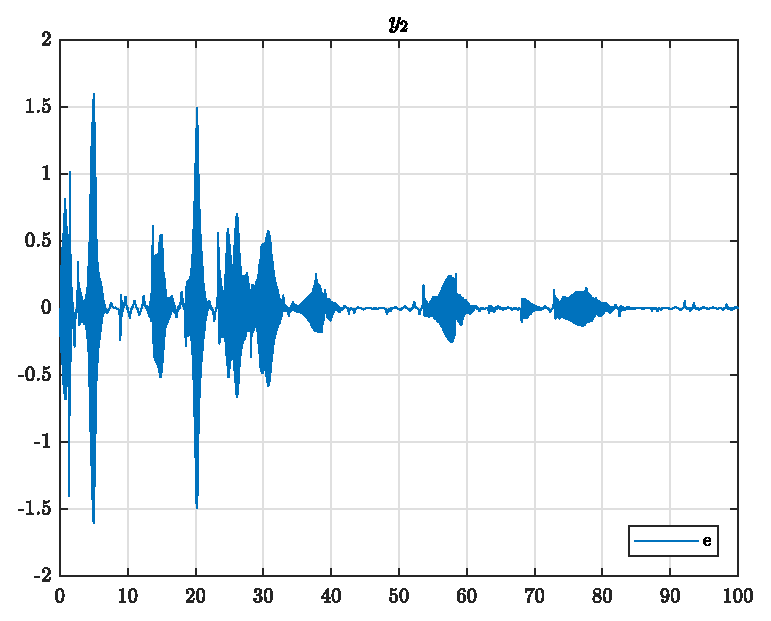
\includegraphics[width=12cm]{figs/en2yp2.eps} 
\end{figure}

\begin{figure}[H]
  \centering
  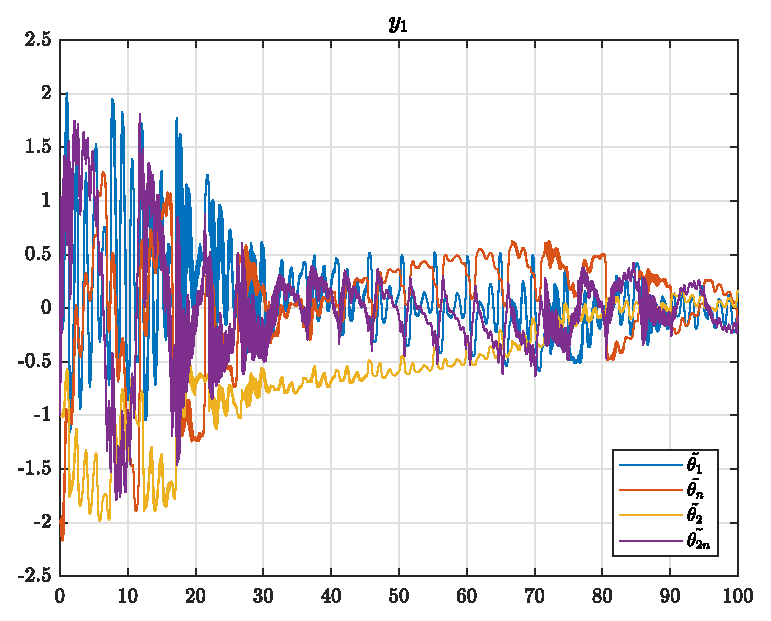
\includegraphics[width=12cm]{figs/tiln2yp1.eps} 
\end{figure}

\begin{figure}[H]
  \centering
  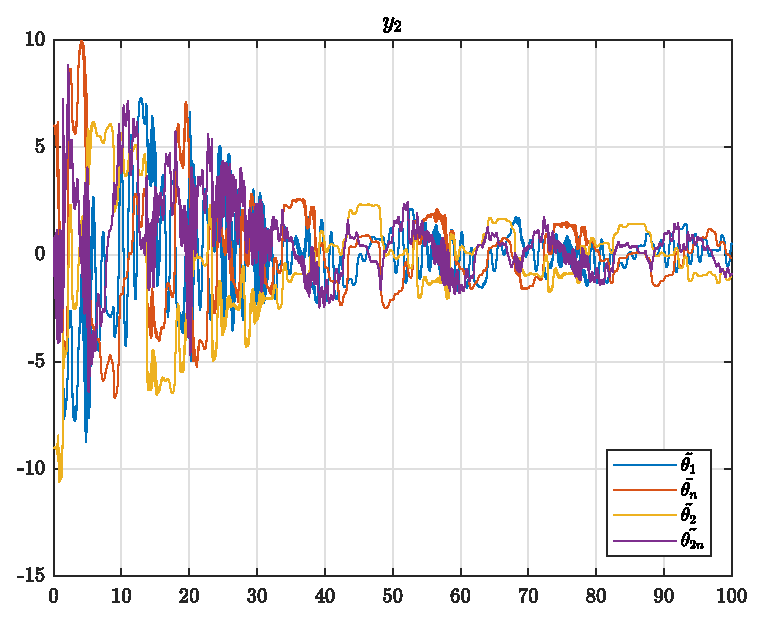
\includegraphics[width=12cm]{figs/tiln2yp2.eps} 
\end{figure}

\textbf{\underline{Simula��o 3.2}: sistema de 3$^\text{a}$ ordem, planta}

\textbf{\underline{Simula��o 3.3}: sistema de 2$^\text{a}$ ordem, modelo}
%
\begin{align*}
  y &= \frac{s+1}{s^2+4s+4}u\, &  y_m &=
  \frac{1}{s+1}r\, \text{e} \frac{1}{s+5}r\,,  & \Lambda &= s+1,\\ \theta(0) &=
  0 \,, & y(0) &= 0 \,, & \gamma &= 20 \, \textbf{I}_4\,, \\ r &=
  10\textrm{sin}(0.63t) + 25\textrm{sin}(4.5t) \, .
\end{align*}
 
\begin{figure}[H]
  \centering
  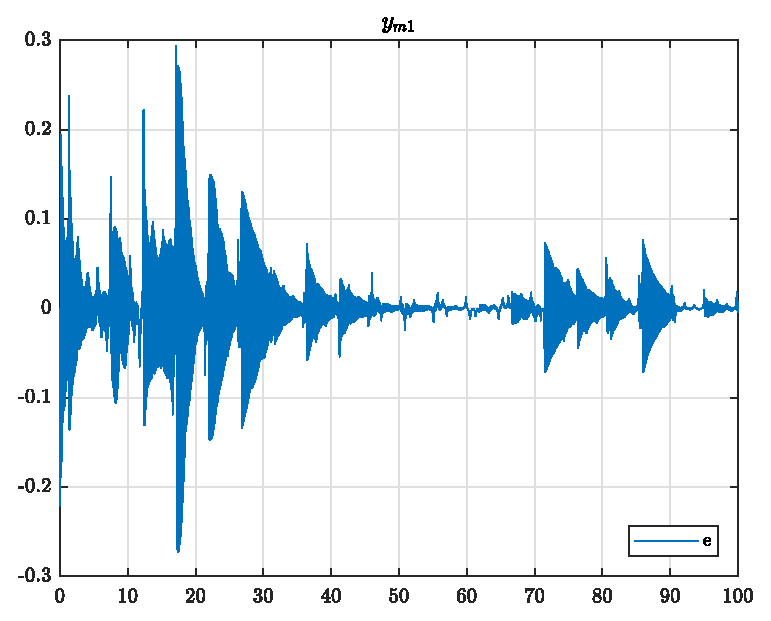
\includegraphics[width=12cm]{figs/en2ym1.eps} 
\end{figure}

\begin{figure}[H]
  \centering
  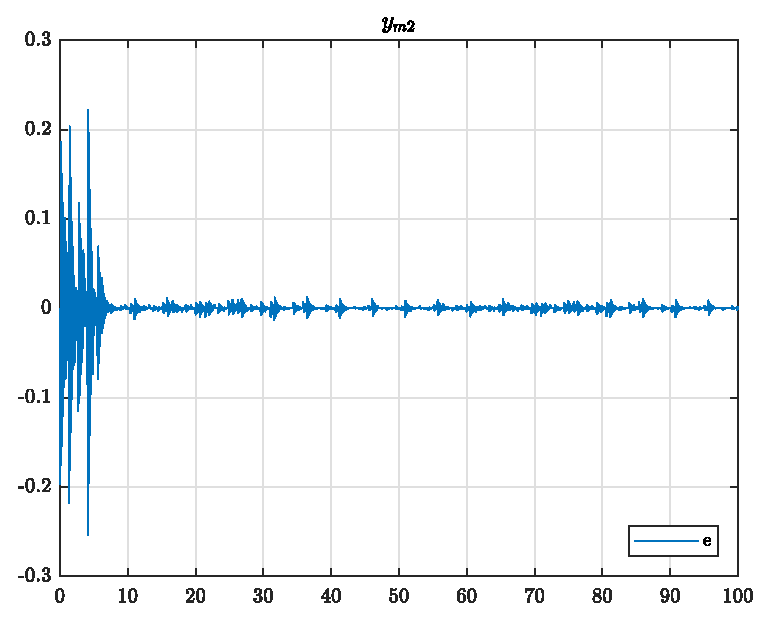
\includegraphics[width=12cm]{figs/en2ym2.eps} 
\end{figure}

\begin{figure}[H]
  \centering
  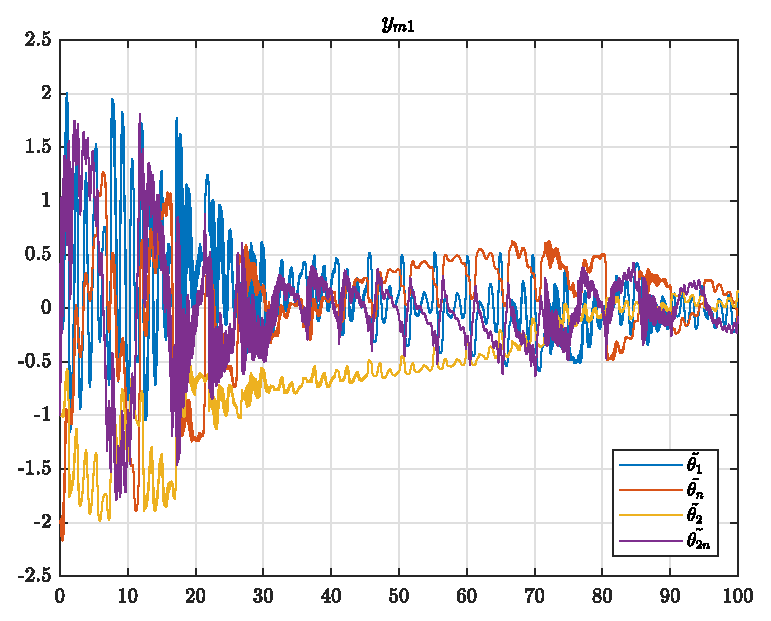
\includegraphics[width=12cm]{figs/tiln2ym1.eps} 
\end{figure}

\begin{figure}[H]
  \centering
  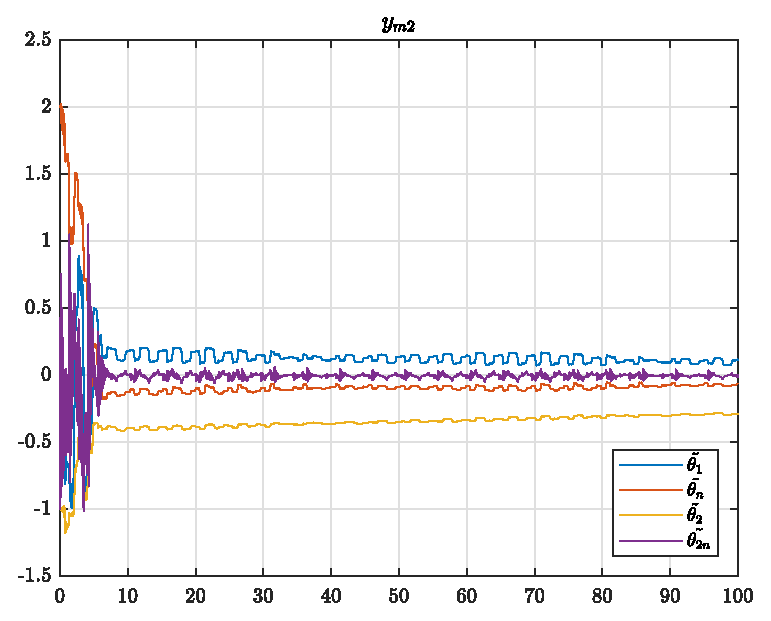
\includegraphics[width=12cm]{figs/tiln2ym2.eps} 
\end{figure}

\textbf{\underline{Simula��o 3.4}: sistema de 3$^\text{a}$ ordem, modelo} \newpage
%---------------------------------------------------------------------
\section{Discuss�o}

% A \textbf{simula��o \#1} mostra o comportamento do sistema para varia��es no sinal de refer�ncia. Como esperado e demonstrado na se��o 3.5 do livro \textit{Adaptive
% Control Design and Analysis} de Gang Tao, a converg�ncia dos par�metros s� �
% garantida quando o sinal de refer�ncia possui o mesmo n�mero de
% frequ�ncias que o n�mero de par�metros desconhecidos (excita��es persistentes).
% 
% Na simula��o 1.1, o sistema � de primeira ordem com dois
% par�metros desconhecidos. Logo, s�o necess�rias duas frequ�ncias diferentes no
% sinal de refer�ncia para garantir que o erro de estima��o $\tilde{\theta}$
% convirja para zero. Isso � verificado, j� que $\tilde{\theta}$ converge para
% zero quando $r=1+5\textrm{sin}(t)$ (frequ�ncia em $\omega=0, \omega=1,
% \omega=-1$) e n�o converge para zero quando o sinal possui apenas uma frequ�ncia
% ($r=1$). Um comportamento semelhante � verificado para os sistemas de segunda e
% terceira ordens (simula��es 1.2 e 1.3, respectivamente). Vale observar que, em
% todos os casos, $\epsilon = \tilde{\theta}^\intercal \phi$ converge para zero,
% como � provado por Lyapunov.  Isso significa que, apesar de a estima��o dos
% par�metros n�o ter garantia de converg�ncia para zero, os vetores $\tilde{\theta}$ e $\phi$ entram em quadratura, ou seja, ficam ortogonais.
% 
% A \textbf{simula��o \#2} mostra o comportamento do sistema para varia��es no
% ganho de adapta��o $\Gamma$ para o m�todo do gradiente normalizado. Nesse caso, a varia��o da estima��o de par�metros � descrita pela f�rmula: $\dot{\theta}(t) = -\Gamma \, \phi(t) \, \epsilon(t) / m^2(t)$. Portanto, a varia��o � proporcional ao ganho de adapta��o, quanto maior o par�metro, mais r�pida ser� a estima��o. J� no caso do m�todo \textit{least-squares} normalizado, o valor inicial do ganho n�o impacta muito no regime transit�rio.
% 
% A \textbf{simula��o \#3} mostra o comportamento do sistema para varia��es nas condi��es iniciais. A rapidez da converg�ncia depende de qu�o pr�ximo os par�metros estimados est�o dos par�metros reais. Na simula��o 3.1, por exemplo, a converg�ncia � mais r�pida quando $\theta = \textbf{0}, \theta^* = \left[1 \, -1\right]$, por�m, na simula��o 3.3, ela � mais r�pida quando $\theta = \textbf{1}$, pois $\theta^* = \left[1 \, 1 \, 1 \, 0 \, 2 \, 2\right]$.
% 
% Observe que o comportamento dos sistemas � semelhante para ambos os m�todos
% utilizados: \textit{Gradiente normalizado} e \textit{least-square
% normalizado}. Pode ser provado que o m�todo \textit{Gradiente
% normalizado} garante converg�ncia exponencial do erro para zero (Tao 3.5.2). J� o m�todo \textit{least-square normalizado} apenas garante converg�ncia, mas n�o
% exponencial (Tao 3.5.3).
% 
% Tamb�m foi constatada, mas n�o relatada aqui, a interessante propriedade do m�todo \textit{least-square normalizado} em que $P^{-1} \, \tilde{\theta} = P_0^{-1} \, \tilde{\theta}(0) = \text{constante} \,$. 
%---------------------------------------------------------------------
%\bibliographystyle{agsm}
%\bibliography{bib,coe736}

%---------------------------------------------------------------------
\end{document}
